\myChapter{Esperimenti}
\label{chap:examples}

\section{Dataset}
\label{sec:dataset}
Inizialmente i dataset usati per gli esperimenti sono due. Il primo è \ac{kmpd} \cite{DBLP:conf/cvpr/HwangPKCK15}, 
per cui è disponibile un'ampia documentazione, il secondo è un dataset gratuito realizzato dalla FLIR \cite{FLIRAdas} per cui è disponibile una documentazione molto stringata.
\subsection{\acl{kmpd}}
\label{subsec:kmpd}
Il \ac{KAIST} propone in \cite{DBLP:conf/cvpr/HwangPKCK15} un dataset che fornisce coppie di immagini termiche e a colori. La particolarità che offre questo dataset è che le due immagini sono allineate. Inoltre sono state raccolte sufficienti immagini sia diurne che notturne.
\paragraph{Specifiche hardware}
\ac{KAIST} ha sviluppato una piattaforma basata su una camera a colori, una termica ed un \textit{Beam Splitter}, oltre che ad un supporto a tre assi chiamato \textit{camera jig}. Un \textit{Beam Splitter} è un dispositivo ottico di forma cubica formato in molti casi da due prismi che divide la luce in due parti. In questo caso viene utilizzato per l'allineamento delle due immagini in quanto permette il passaggio dello spettro termico mentre quello visibile viene riflesso. Il dispositivo usato per la realizzazione del dataset è stato costrutito a partire da un wafer di silicio zincato.

Le telecamere utilizzate sono una \textit{PointGrey Flea3} per la parte a colori ed una \textit{FLIR-A35} per la parte termica. La prima acquisisce immagini ad una risoluzione di $640 x 480$ pixels con un \ac{FOV} di $103.6^\circ$, mentre la seconda ha una risoluzione di $320 x 256$ con un un \ac{FOV} di $39^\circ$. Come si può notare il campo visivo della telecamera visibile è più ampio di quello della telecamera termica, motivo per cui viene sacrificata parte dell'immagine visibile al fine di allineare i due fotogrammi. Il \textit{framerate} è di $20$ FPS.
\paragraph{Calibrazione} L'idea per la realizzazione di questa architettura hardware è stata ripresa dal lavoro di Bienkowski \textit{et al.} \cite{bienkowski2012}. Sempre in questo lavoro però non si fa riferimento alla metodologia usata per la calibrazione. Parleremo in questo paragrafo dell'approccio utilizzato per la realizzazione di questo dataset. Innanzitutto è stata calcolata la traslazione fra le due telecamere, applicando la calibrazione stereo. Si può osservare che gli assi ottici delle telecamere al di là della divisione del fascio di luce sono paralleli a causa delle impostazioni tecniche. Di conseguenza, fra i due domini dell’immagine, è presente unicamente una traslazione ed è necessario solamente aggiustare la posizione tramite \textit{camera jig} a tre assi finché la traslazione non diventa nulla. Dopo l’aggiustamento, i due domini sono rettificati fino ad avere la stessa distanza focale virtuale. Al termine di queste procedura, oltre alla focale, i domini condividono i punti principali e sono privi di baseline.
Il dominio dell’immagine, virtualmente allineato, ha $640 x 512$ pixel di risoluzione spaziale e un \ac{FOV} di $39^\circ$, analogamente a quella umano. Visto che un pattern a scacchiera convenzionale non è osservabile con telecamera termica, viene invece utilizzata una tavola di calibrazione speciale, con un certo numero di buchi. Quando viene scaldata, si ottiene una differenza di temperatura fra la tavola e i buchi, che possono essere osservati nel termico.
\paragraph{Correzione dei colori}
Per via del passaggio all'interno dei prismi del \textit{Beam Splitter} le immagini catturate, soprattutto nello spettro del visibile, mostrano distorsioni piuttosto evidenti dei colori. Per gestire questo problema è stato deciso di acquisire un fotogramma di riferimento completamente bianco che mostrava distorsioni di colore. Per motivi legati al sensore utilizzato all'interno della telecamera visibile la distorsione del colore può essere considerata come una funzione lineare. Quindi ogni pixel dell'immagine di riferimento può essere usato come coefficente di correzione per le altre immagini, dividendo il livello di intensità di queste immagini per questi coefficenti.
\paragraph{Acquisizione dei dati e annotazioni}
Tutto il marchingegno composto dalle due telecamere, il \textit{Beam Splitter} ed il \textit{Camera jig} è stato montato sul tetto di un'automobile al fine di realizzare immagini egocentriche del traffico. In particolare, come già accennato in precedenza, sono state realizzate raccolte di dati sia di giorno che di notte.

Il numero totale delle coppie di immagini catturate sono $95328$ le quali sono state annotate manualmente con un totale di $103128$ \ac{BB}. Per realizzare le annotazioni è stata usata una versione modificata del Piotr's Computer Vision Toolbox \cite{PMT}. Le \ac{BB} sono state annotate con quattro differenti label:
\begin{itemize}
    \item \texttt{person}: individuo singolo ben individuabile
    \item \texttt{people}: individui non distinguibili
    \item \texttt{cyclist}: persone che stanno utilizzando una bicicletta
    \item \texttt{person?}: individuo non ben identificabile per via di fotogrammi molto densi
\end{itemize}
Inoltre, anche se per lo scopo della tesi non sono stati presi in considerazione, ogni \ac{BB} ha una corrispondenza temporale che identifica il singolo individuo attraverso i vari frame.
\paragraph{Train e test set}
Per dividere tra \textit{train set} e \textit{test set} è stato usato un criterio ben definito:
\begin{itemize}
    \item Il numero di pedoni nei due set è simile
    \item Il numero di frame notturni e diurni nei due set è simile
    \item I due set non si sovrappongono
\end{itemize}
\paragraph{Proprieta}
\begin{itemize}
    \item Attributo di scala: per ogni \ac{BB} è associato un valore di scala. Questo valore dipende dalla distanza che ha il pedone dall'automobile, ed è giustificato dalla seguente affermazione. Supponendo che una vettura in area urbana viaggia ad una velocità compresa tra $30$ e $50$ km/h lo spazio di arresto varia tra gli $11$ ed i $28$ metri. Questo intervallo, scalato opportunamente rispetto alla risoluzione dell'immagine, e considerando anche che l'altezza media di un pedone è di $1.7$ metri corrisponde ad un range che va da $45$ a $115$ pixel. All'interno di questo range vengono definite \textit{medium}, al di sopra \textit{far} ed al di sotto \textit{near}.
    \item Occlusione: questo attributo associa ad ogni \ac{BB} un valore che rappresenta l'occlusione del pedone. I valori possibili sono \textit{no occlusion}, \textit{partial occlusion}, \textit{heavy occlusion}. I primi sono circa il $78.6\%$, i secondi circa il $12.6\%$ e gli ultimi $8.8\%$.
    \item Posizione: l'impostazione dell'hardware rispecchia il più possibile quello di un essere umano, motivo per cui questo particolare setup concentra il rilevamento di pedoni nell'area centrale dell'immagine, in particolare nel lato destro. Questo è motivato dal fatto che nel paese dove sono stati acquisiti questi dati la guida è sulla destra. In Figura \ref{fig:heatmap} è possibile vedere questo fenomeno.
    \item Cambio d'aspetto: l'aspetto dei pedoni all'interno del dataset è molto variabile. In condizioni di pieno sole i pedoni sono ben visibili e con dei contorni ben definiti, mentre la differenza di temperatura tra l'ambiente circostante ed il pedone è meno marcata. Quindi nello spettro a colori sono presenti pedoni ben definiti, mentre nel termico no. Di notte invece, per via delle temperature ambientali più basse e per l'assenza di luce si verifica il contrario. In figura \textbf{INSERIRE FIGURA} è presente un esempio.
\end{itemize}
\begin{figure}
    \centering
    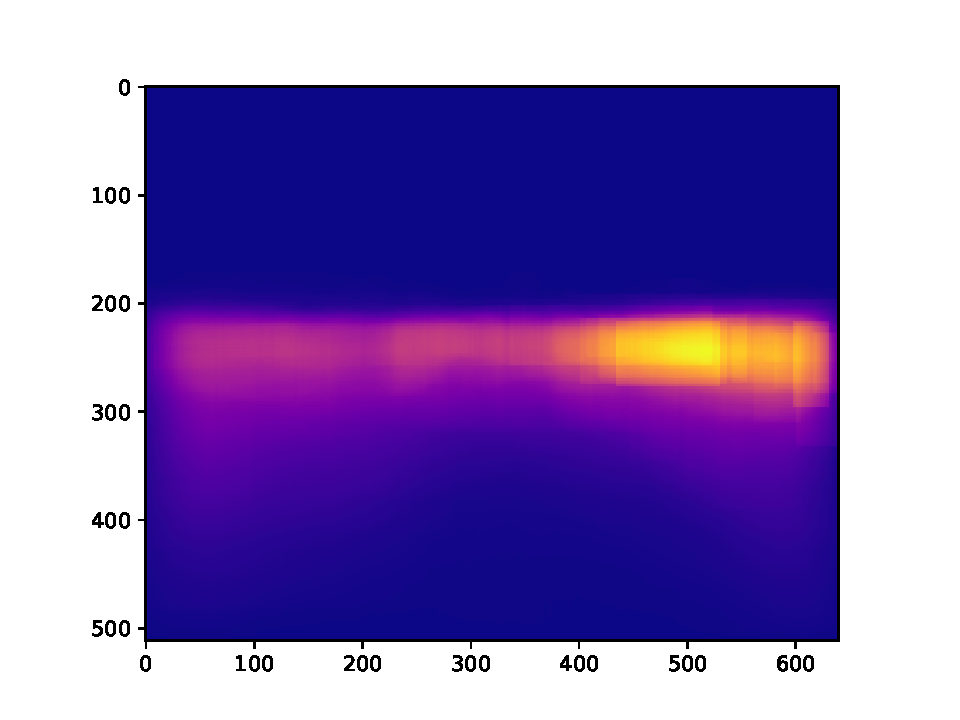
\includegraphics[width=0.8\textwidth]{images/graphic/heatmap.pdf}
    \caption{Heatmap riguardante la posizione dei pedoni}
    \label{fig:heatmap}
\end{figure}
\subsection{FLIR Thermal Starter Dataset}
\label{subsec:flirdataset}
Come già accennato in precedenza la documentazione riguardante questo dataset è molto stringata, limitandosi dunque ad una sola \href{https://www.flir.com/oem/adas/adas-dataset-form/}{pagina web} molto riassuntiva. Cercheremo in questa sezione di parlare degli aspetti che caratterizzano questo dataset.

Il dataset in questione offre immagini termiche con annotazioni e l'equivalente a colori non annotato. A differenza di \ref{subsec:kmpd} le due immagini non sono allineate, quindi non è possibile portare le annotazioni delle immagini termiche sulle immagini a colori.
Le immagini sono state acquisite tramite telecamere montate su una vettura e contiene un totale di 14453 immagini, di cui 10228 campionate da video di breve durata e 4224 provenienti da video di 144 secondi.
Tutte le immagini sono state acquisite su strade ed autostrade a Santa Barbara, in California. L'arco temporale varia da Novembre a Maggio, nello stessa quantità di giorno e notte. Il meteo è generalmente buono.

Le immagini termiche sono state scattate con una \textit{FLIR Tau2}, mentre quelle RGB con una \textit{FLIR BlackFly}. Entrambi i device sono stati impostati in maniera tale da avere lo stesso \ac{FOV} e per quanto riguarda il resto sono state lasciate entrambe alle impostazioni di default. 
Le videocamere sono state posizionate sullo stesso supporto a distanza di circa $1.9$ pollici (circa $4.8$ centimetri) l'una dall'altra. Il \textit{framerate} è di $2$ frame al secondo in scenari densi di annotazioni, mentre in scenari più tranquilli è stato deciso di scendere ad un frame al secondo.

Le annotazioni dove possibile ricalcano i codici adottati dal dataset \href{http://cocodataset.org/}{COCO}, ed hanno i seguenti codici:
\begin{itemize}
    \item 1 People: esseri umani.
    \item 2 Bicycles: biciclette e moticicli. Questa è l'unica categoria non consistente con il formato adottato da COCO.
    \item 3 Cars: automobili e veicoli piccoli.
    \item 18 Dogs: cani 
    \item 91 Other Vehicle: camion, rimorchi e imbarcazioni.
\end{itemize}

Le annotazioni sono state fatte manualmente da esseri umani ai quali è stato comunicato di fare \ac{BB} il più piccole possibili e che omettessero piccole parti di oggetti, accessori personali e parti occluse. Inoltre è stato comunicato di non annotare oggetti di piccole dimensioni o molto occlusi e persone delle quali si vede solo braccia o gambe.

\section{Addestramento iniziale di RetinaNet}
\label{sec:addestramento_iniziale_di_retinanet}
In questa sezione presenteremo i risultati iniziali dell'addestramento di RetinaNet sui due dataset descritti in sezione \ref{sec:dataset}. Per lo scopo è stata usata una versione di \textit{RetinaNet} implementata tramite \textit{Keras} reperibile in forma originale al seguente \href{https://github.com/fizyr/keras-retinanet}{link}. Durante lo sviluppo del lavoro di tesi le modifiche al codice originale sono state molteplici, tanto da aver richiesto un \textit{fork} della \textit{repository} originale reperibile al seguente \href{https://github.com/iskorini/keras-retinanet}{link}. Per tenere traccia dell'addestramento è stato usato \href{https://www.wandb.com}{\textit{Weight \& Biases}}.
\subsection{Transfer Learning}
\label{subsec:transfer_learning}
Inizialmente è stata usata la tecnica del \textit{Transfer Learning}. Una rapida spiegazione del significato di questa espressione ce la fornisce il libro \textit{Deep Learning} di \textit{Goodfellow et al} \cite{Goodfellow-et-al-2016}
\begin{quote}
    Transfer learning and domain adaptation refer to the situation where what has been learned in one setting is exploited to improve generalization in another setting.
\end{quote}
Per un'introduzione più dettagliata su cos'è il \textit{transfer learning} e sui vari tipi è stato preso spunto da \textit{A survey on Transfer Learning} di \textit{S. J. Pan} e \textit{Q. Yang} \cite{5288526}. 

La necessità di attuare tecniche di \textit{transfer learning} deriva dal fatto che molti modelli di Machine Learning lavorano bene solo sotto determinate assunzioni, soprattutto quella che i dati di addestramento e di test derivino dallo stesso spazio delle \textit{feature} e dalla stessa distribuzione. I problemi sorgono quando cambia la distribuzione, in quanto è necessario procedere ad una nuova fase di training. 

Le casistiche in cui il \textit{transfer learning} è applicabile sono molteplici, ad esempio l'analisi dei sentimenti, dove il compito è classificare le recensioni di un determinato prodotto in positive o negative. Per un compito del genere il primo passo da effettuare è la raccolta e l'annotazione di recensioni. Successivamente è necessaria una fase di addestramento di un modello usando come dati le recensioni precedentemente raccolte ed annotate.
Lo scopo è poter usare lo stesso modello per vari prodotti, in questo caso però si va incontro al problema che le distribuzioni dei dati su diversi prodotti possono differire anche di molto. La soluzione sarebbe quindi di annotare altre recensioni, ma richiederebbe uno sforzo notevole. L'idea è quindi di adattare un modello di classificazione, addestrato su alcuni prodotti, per aiutare la fase di addestramento su articoli differenti.
Le differenze tra processi di apprendimento tradizionali e \textit{transfer learning} sono mostrate in Figura \ref{fig:differences}.
\begin{figure}.
    \centering
    \subfloat[\label{fig:differencesa}]{
    \begin{tikzpicture}
        \node[circle, draw, ultra thick, fill=gray!20, minimum size=1.6cm](task1) {Task 1};
        \node[circle, draw, ultra thick, fill=gray!20, right = 0.7cm of task1, minimum size=1.6cm](task2) {Task 2};
        \node[circle, draw, ultra thick, fill=gray!20, right = 0.7cm of task2, minimum size=1.6cm](task3) {Task 3};
        \node[rectangle, draw, ultra thick, fill=gray!20, below = 1.5cm of task1](m1) {Modello};
        \node[rectangle, draw, ultra thick, fill=gray!20, below = 1.5cm of task2](m2) {Modello};
        \node[rectangle, draw, ultra thick, fill=gray!20, below = 1.5cm of task3](m3) {Modello};
        \draw[vecArrow] (task1) to (m1);
        \draw[vecArrow] (task2) to (m2);
        \draw[vecArrow] (task3) to (m3);
    \end{tikzpicture}
    \label{fig:differencesa}
    }
    \subfloat[\label{fig:differencesb}]{
    \begin{tikzpicture}[]
        \node[circle, draw, ultra thick, fill=gray!20, minimum size=1.6cm](task1) {Task 1};
        \node[circle, draw, ultra thick, fill=gray!20, right = 0.7cm of task1, minimum size=1.6cm](task2) {Task 2};
        \node[circle, draw, ultra thick, fill=gray!20, right = 0.7cm of task2, minimum size=1.6cm](task3) {Task 3};
        \path (task1) -- (task2) node[rectangle, draw, ultra thick, fill=gray!20, pos=.5,below=2.4cm] (m1) {Conoscenza};
        \node[rectangle, draw, ultra thick, fill=gray!20, below of = task3, right of = m1](m3) {Modello};
        \draw[vecArrow] (task1) to (m1);
        \draw[vecArrow] (task2) to (m1);
        \draw[vecArrow] (task3) to (m3);
        \draw[vecArrow] (m1) to (m3);
        \end{tikzpicture}
    }
    
    \caption{Differenze tra apprendimento tradizionale e transfer learning}
    \label{fig:differences}
\end{figure}

\paragraph{Notazione preliminare}
Per introdurre un po' più nello specifico le varie tipologie di \textit{transfer learning} è necessario definire alcuni concetti. Il primo di questi è il \textit{Dominio} $\mathcal{D}$, definito come una tupla $\mathcal{D} = \{\mathcal{X}, P(X)\}$, dove $\mathcal{X}$ è lo spazio delle \textit{feature} e $P(X) \text{ con } X = \{x_1, x_2, \dots, x_n\} \in \mathcal{X}$ è una distribuzione di probabilità marginale. In generale due domini possono essere considerati differenti se hanno differenti spazi delle \textit{feature} o distribuzioni differenti. 

Dato uno specifico dominio $\mathcal{D} = \{\mathcal{X}, P(X)\}$ è possibile definire il \textit{task}. Un \textit{task} $\mathcal{T}$ è una tupla $\mathcal{T} = \{\mathcal{Y},f(\cdot)\}$ con $\mathcal{Y}$ spazio dei \textit{label} e $f(\cdot)$ funzione di predizione. La particolarità del \textit{task} è il fatto che non è osservabile ma può essere appreso dai dati di addestramento, che consistono di una coppia $\{x_i, y_i\}$ con $x_i \in X$ e $y_i \in \mathcal{Y}$. Una volta completata la fase di addestramento dovrebbe essere possibile usare la funzione $f(\cdot)$ per predirre il label $f(x)$ corrispondente ad una nuova istanza $x$.

Chiameremo il dominio sorgente $\mathcal{D}_S$ ed il dominio target $\mathcal{D}_t$. In particolare avremo a disposizione anche i dati $D_S$ del dominio sorgente, definiti 
come $D_S = \{(x_{S_1}, y_{S_1}), \dots, (x_{S_n}, y_{S_n})\}$ tali che $x_{S_i} \in \mathcal{X}_S$ è l'istanza del dato e $y_{S_i} \in \mathcal{Y}_S$ è il corrispondente label. In maniera similare definiamo anche i dati del dominio target $D_T = \{(x_{T_1}, y_{T_1}), \dots, (x_{T_n}, y_{T_n})\} $ tali che $x_{T_i} \in \mathcal{X}_T$ è l'istanza del dato e $y_{T_i} \in \mathcal{Y}_T$ è il corrispondente label. 

Dire che due domini $\mathcal{D}_S$ e $\mathcal{D}_T$ implica che  o $\mathcal{X}_S \neq \mathcal{X}_T$ oppure $P_X(X) \neq P_T(X)$. In maniera del tutto analoga è possibile definire la differenza tra due \textit{task} $\mathcal{T}_S \text{ e } \mathcal{T}_T$. Nel caso in cui i due domini ed i due task sono uguali ci si riconduce ad un tradizionale problema di apprendimento. Quando invece c'è una relazione, implicita o esplicita, tra gli spazi delle \textit{feature} dei due domini si dice che il dominio sorgente e target sono in relazione tra di loro.
\paragraph{Tipologie di Transfer Learning} Prima di introdurre le varie tipologie di \textit{transfer learning} è necessario definire formalmente questo concetto e fare alcune premesse.
\begin{definition}{(Transfer Learning)}
    Dato un dominio sorgente $\mathcal{D}_S$, un task di apprendimento $\mathcal{T}_S$, un dominio target $\mathcal{D}_T$ ed un task di apprendimento $\mathcal{T}_T$, il transfer learning tenta di migliorare l'apprendimento di $f(\cdot)_T \in \mathcal{D}_T$ usando la conoscenza in $\mathcal{D}_S$ e $\mathcal{T}_S$, con $\mathcal{D}_S \neq \mathcal{D}_T$ o $\mathcal{T}_S \neq \mathcal{T}_T$.
\end{definition}
Quando si parla di \textit{transfer learning} bisogna mettere in conto tre problemi: \emph{cosa}, \emph{come} e \emph{quando} trasferire.
\begin{itemize}
    \item Cosa trasferire: quale parte della conoscenza bisogna trasferire tra domini o task sorgenti e target. In particolare possiamo dire che alcune conoscenze sono comuni tra i diversi domini, mentre altre sono specifiche. 
    \item Come trasferire: a questo problema pone una soluzione l'algoritmo di trasferimento della conoscenza.
    \item Quando trasferire: ci chiediamo in quali situazioni è realmente necessario applicare tecniche di \textit{transfer learning} ed in quali non è assolutamente necessario. Ad esempio in casi in cui i due domini sorgente e target non sono in relazione tra di loro il \textit{transfer learning} potrebbe non portare ad alcun risultato positivo. Si tende quindi sempre a parlare di \textit{transfer learning} dando per scontato che i due domini siano in qualche modo relazionati tra di loro, in quanto altrimenti non avrebbe senso andare oltre l'apprendimento tradizionale. 
\end{itemize}

Possiamo ora descrivere le tre categorie di \textit{transfer learning}:
\begin{itemize}
    \item \emph{Transfer Learning Induttivo}: il task target è differente dal task sorgente e non importa se il dominio sorgente ed il dominio target sono uguali o meno. Per indurre un modello predittivo oggettivo, da usare nel dominio target, sono necessari alcuni dati etichettati nel dominio sorgente. A seconda della tipologia ed alla quantità di annotazioni possiamo dividere questo tipo di \textit{transfer learning} in ulteriori due sottocategorie.
    \begin{itemize}
        \item Molti dati annotati nel dominio sorgente: ci si riconduce al caso del \textit{multitask learning}, tuttavia mentre lo scopo di quest'ultimo è operare bene in entrambi i domini, lo scopo del \textit{transfer learning} induttivo è operare bene solamente sul dominio obbiettivo.
        \item Nessun dato annotato nel dominio sorgente: le similarità in questo caso ci portano a pensare al \textit{self-taught learning}, dove le annotazioni tra il dominio sorgente ed obbiettivo sono totalmente differenti, e quindi non direttamente utilizzabili. 
    \end{itemize}
    \item \emph{Transfer Learning Trasduttivo (si traduce così "transductive"?)}: in questo caso il task obbiettivo ed il task sorgente sono i medesimi, mentre i domini sono differenti. Abbiamo quindi molti dati annotati nel dominio sorgente e nessuna annotazione nel dominio obbiettivo. Possiamo a sua volta dividere questa categoria in ulteriori due sottocategorie.
    \begin{itemize}
        \item Gli spazi delle feature tra sorgente e obbiettivo sono diffrenti, più formalmente abbiamo $\mathcal{X}_S \neq \mathcal{X}_T$
        \item Gli spazi delle feature tra sorgente e obbiettivo sono gli stessi, ma cambia la distribuzione di probabilità marginale, quindi $P(X_S) \neq P(X_T)$. Quest'ultimo caso è chiamato anche \emph{Domain Adaptation}.
    \end{itemize}
    \item \emph{Transfer Learning non supervisionato}: il task obbiettivo è differente dal task sorgente, ma hanno una qualche tipo di relazione tra di loro. Tuttavia l'attenzione si focalizza sul risolvere compiti di apprendimento non supervisionati nel dominio obbiettivo, come possono essere il \textit{clustering}, \textit{dimensionality reduction} o \textit{density estimation}. Non abbiamo quindi annotazioni né nel dominio sorgente, né nel dominio obbiettivo.
\end{itemize}
In Tabella \ref{table:TransferLearning} sono riassunte tutte le caratteristiche principali delle varie categorie di \textit{transfer learning}.
%TODO: SISTEMARE TABELLA
\textbf{SISTEMARE TABELLA \ref{table:TransferLearning}}
\begin{table}[]
    \centering
    \makebox[\textwidth]{
    \begin{tabular}{|c|c|c|c|c|}
    \hline
    Tipologia          & Similarità           & Annotazioni Sorgente & Annotazioni Target & Campo di applicabilità               \\ \hline
    Induttivo          & Multitask Learning   & SI                           & SI                         & Regressione e Classificazione        \\ \cline{2-5} 
                       & Self-taught Learning & NO                           & SI                         & Regressione e Classificazione        \\ \hline
    Trasduttivo        & Domain adaptation    & SI                           & NO                         & Regressione e Classificazione        \\ \hline
    Non supervisionato & 46501                & NO                           & NO                         & Clustering, dimensionality reduction \\ \hline
    \end{tabular}}
    \caption{Schema riassuntivo delle categorie di Transfer Learning}
    \label{table:TransferLearning}
\end{table}
\subsection{Addestramento sulle immagini RGB}
\label{subsec:first_training_rgb_kaist}
Per il primo esperimento è stato deciso di effettuare un training di \textit{RetinaNet} partendo dai pesi della rete precedentemente addestrata sul dataset di \href{http://cocodataset.org/}{COCO}. Il dataset utilizzato è \ac{kmpd}, descritto precedentemente in \ref{subsec:kmpd}. Il motivo è legato al fatto che è l'unico dataset a nostra disposizione a disporre di annotazioni sulle immagini RGB.

Questa prima fase di addestramento è durata circa $40$ ore, e come si può vedere dal grafico in Figura \ref{fig:fine_tuning_1} è proceduta senza particolari problemi fino ad arrivare a convergenza intorno all'epoca 45. Le classi usate per l'addestramento sono solamente \textit{person} e \textit{cyclist}. È stato deciso di non prendere in considerazioni le rimanenti classi in quanto sono persone non ben distinguibili. Tutti gli esperimenti sono stati eseguiti su una macchina remota dotata di una \ac{gpu} \href{https://www.geforce.com/hardware/desktop-gpus/geforce-gtx-titan-x}{Nvidia Titan X}.

\begin{figure}[h]
    \centering
    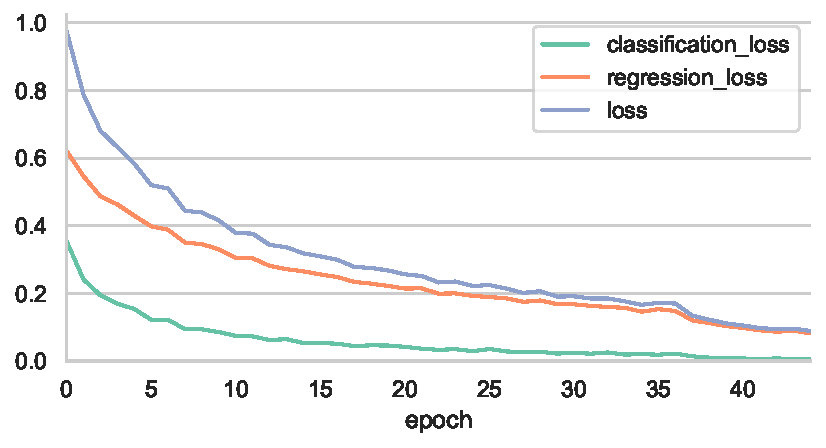
\includegraphics[width=\textwidth]{images/graphic/ruby-yogurt.pdf}
    \caption{Transfer learning da COCO a KAIST}
    \label{fig:fine_tuning_1}
\end{figure}

Dopo la fase di addestramento sono stati eseguite le valutazioni sulla parte di dataset adibita ai test. Inizialmente le classi utilizzate per i test sono le stesse usate per l'addestramento. I risultati complessivi vengono riassunti in Tabella \ref{table:first_test}. La \ac{map} mostrata nell'ultima riga della tabella è stata calcolata come media pesata secondo il numero di esempi all'interno del \textit{test set}.

\begin{table}[]
    \centering
    \begin{tabular}{|c|c|c|}
    \hline
                & $\#$ Istanze & mAP    \\ \hline
    Person      & 45195             & 0.4184 \\ \hline
    Cyclist     & 1396              & 0.1154 \\ \hline
    Complessivo & 46501             & 0.4093 \\ \hline
    \end{tabular}
    \caption{Test complessivo delle performance dopo l'addestramento}
    \label{table:first_test}
\end{table}

La valutazione è stata anche effettuata in maniera separata sia sulla parte di \textit{test set} diurna che notturna. I risultati sono mostrati in Tabella \ref{table:separate_test_day} e Tabella \ref{table:separate_test_night}. Come lecito aspettarsi, avendo visibilità limitata in notturna si ottengono risultati mediamente peggiori. In Figura \ref{fig:prediction_test_first} è possibile vedere un esempio di predizioni fatte sul \textit{test set}.

\begin{table}[]
    \centering
    \subfloat[Giorno\label{table:separate_test_day}]{
        \begin{tabular}{|c|c|c|}
        \hline
                    & $\#$ Istanze & mAP    \\ \hline
        Person      & 33688             & 0.4493 \\ \hline
        Cyclist     & 818               & 0.2015 \\ \hline
        Complessivo & 34506             & 0.4434 \\ \hline
        \end{tabular}
    }
    \subfloat[Notte\label{table:separate_test_night}]{
        \begin{tabular}{|c|c|c|}
        \hline
                    & $\#$ Istanze & mAP    \\ \hline
        Person      & 11507             & 0.3281 \\ \hline
        Cyclist     & 578               & 0.0029 \\ \hline
        Complessivo & 12085             & 0.3125 \\ \hline
        \end{tabular}
    }
    \caption{Risultati della valutazione separata}
    \label{table:separate_test}
\end{table}

\begin{figure}[]
    \centering
    \makebox[\textwidth]{
    \subfloat{
        \begin{minipage}[b][][t]{.3\textwidth}
        \centering
        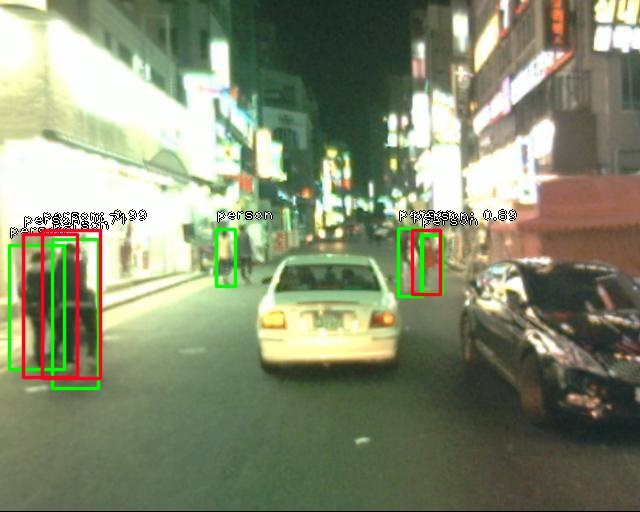
\includegraphics[width=.8\textwidth]{images/examples/first_test/I00011.jpg}
        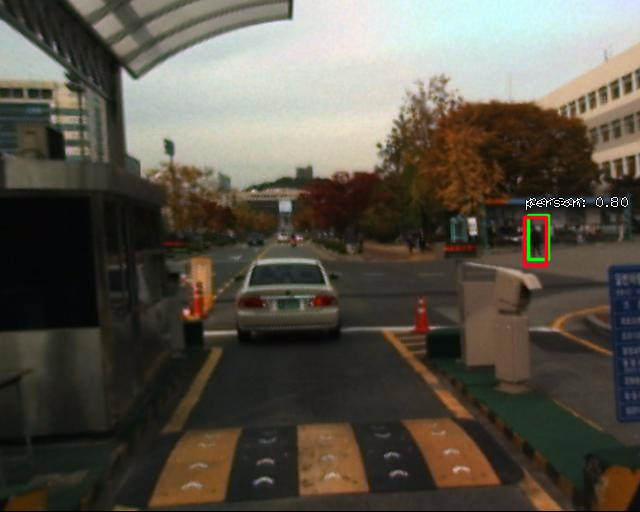
\includegraphics[width=.8\textwidth]{images/examples/first_test/I00146.jpg}
        \end{minipage}
    }%
    \subfloat{
        \begin{minipage}[b][][t]{.3\textwidth}
        \centering
        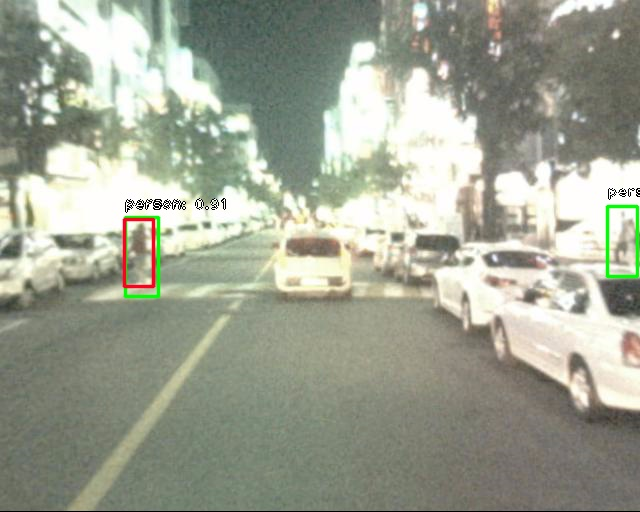
\includegraphics[width=.8\textwidth]{images/examples/first_test/I00222.jpg}
        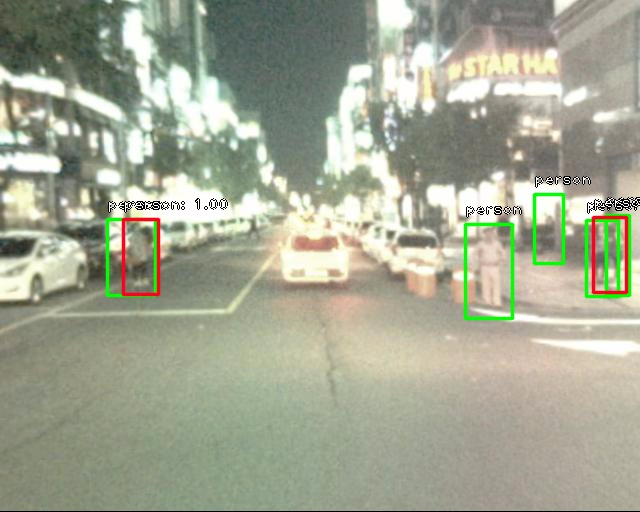
\includegraphics[width=.8\textwidth]{images/examples/first_test/I00159.jpg}
        \end{minipage}
    }
    \subfloat{
        \begin{minipage}[b][][t]{.3\textwidth}
        \centering
        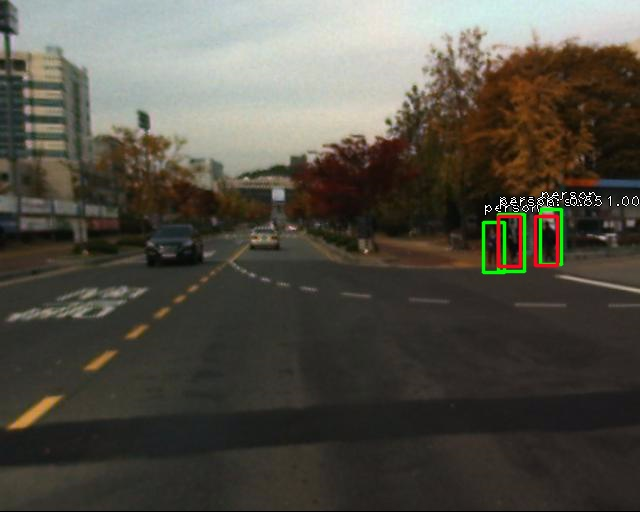
\includegraphics[width=.8\textwidth]{images/examples/first_test/I00265.jpg}
        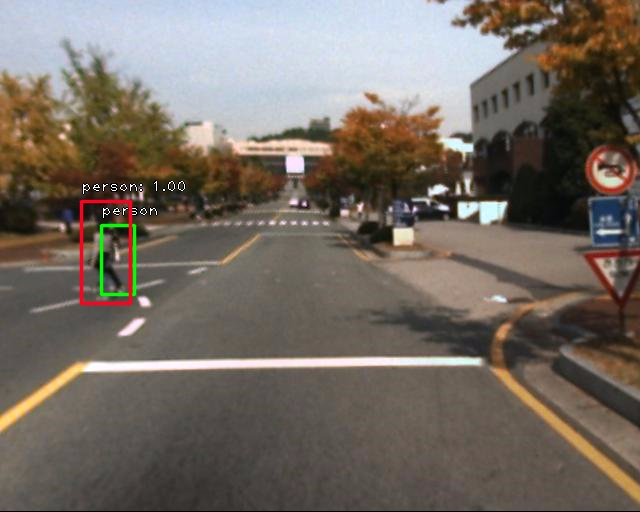
\includegraphics[width=.8\textwidth]{images/examples/first_test/I00599.jpg}
        \end{minipage}
    }
    \subfloat{
        \begin{minipage}[b][][t]{.3\textwidth}
        \centering
        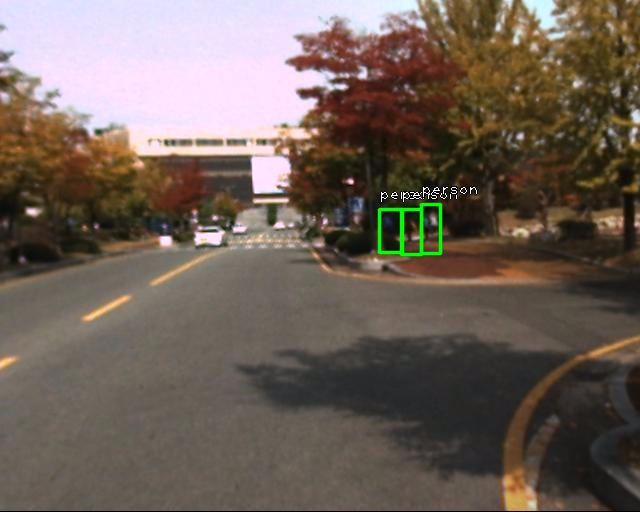
\includegraphics[width=.8\textwidth]{images/examples/first_test/I01314.jpg}
        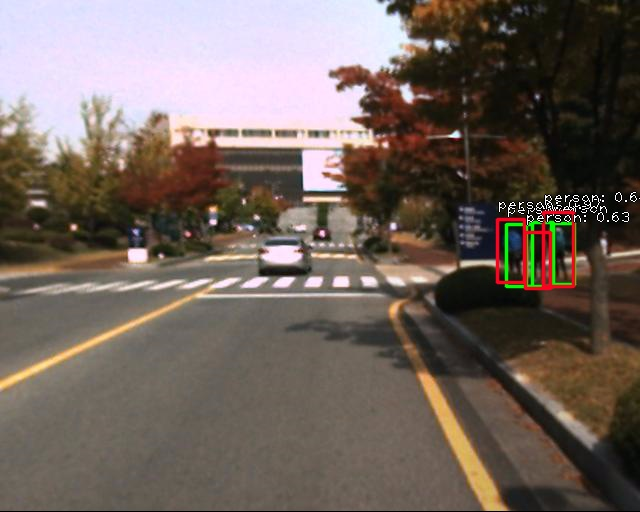
\includegraphics[width=.8\textwidth]{images/examples/first_test/I01512.jpg}
        \end{minipage}
    }
    }
    \caption{Esempio di predizioni, in verde la \textit{ground truth} in rosso le predizioni.} 
    \label{fig:prediction_test_first} 
\end{figure}


Il successivo step della valutazione è stato effettuato su più classi, per questa comparazione delle performance è stata presa in considerazione anche la classe \textit{people}, ma rinominandola in \textit{person} in maniera tale da farla digerire \textbf{rivedere questo periodo} alla rete già addestrata.
\textbf{INSERIRE VALUTAZIONE EFFETTUATA CON TUTTE LE CLASSI, APPENA LE GPU SI LIBERANO. I PESI SONO QUELLI DELLA RUN RUBY-YOGURT}
\subsection{Passaggio alle immagini termiche su KAIST}
Dopo la fase di addestramento descritta in Sezione \ref{subsec:first_training_rgb_kaist} è stato effettuato il passaggio all'addestramento sulle immagini termiche del dataset di \ac{kmpd}. La base di partenza per questa fase di \textit{training} sono i pesi derivanti dall'addestramento effettuato in Sezione \ref{subsec:first_training_rgb_kaist}, è quindi stata attuata una tecnica di \textit{Transfer Learning} (\ref{subsec:transfer_learning}) in maniera da ridurre i tempi di addestramento. In questo caso, operando su due tipologie di immagini differenti cambia il dominio, più in particolare lo spazio delle feature. La distribuzione di probabilità sulle varie immagini resta la medesima in quanto il training è svolto sulle stesse immagini, come rimane invariato anche il task, ovvero il riconoscimento di pedoni e ciclisti.
La fase di apprendimento è proceduta senza particolari intoppi, come si può vedere in Figura \ref{fig:fine_tuning_2} le varie loss scendono in maniera stabile e controllata. In maniera del tutto similare a quanto si può vedere in Figura \ref{fig:fine_tuning_1}.

\begin{figure}[]
    \centering
    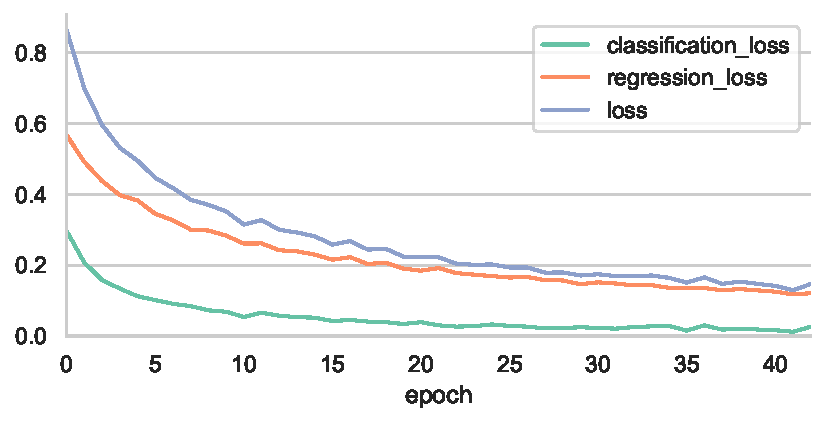
\includegraphics[width=\textwidth]{images/graphic/ruby-yogurt-lwir.pdf}
    \caption{Transfer learning da KAIST Visibile a KAIST Termico}
    \label{fig:fine_tuning_2}
\end{figure} 
I risultati della valutazione sul test set sono mostrati in maniera complessiva in Tabella \ref{table:first_test_lwir_kaist}. Il test è stato effettuato usando i label \textit{person}, \textit{cyclist} e \textit{people}, quest'ultimi oppurtunamente rinominati in \textit{person} per farli riconoscere correttamente a RetinaNet. La prima cosa che si nota è un calo delle performance rispetto al test sulle immagini visibili (Tabella \ref{table:first_test}).
\begin{table}[]
    \centering
    \begin{tabular}{|c|c|c|}
    \hline
                & $\#$ Istanze & mAP    \\ \hline
    Person      & 53443             & 0.3663 \\ \hline
    Cyclist     & 1396              & 0.0392 \\ \hline
    Complessivo & 54839             & 0.3580 \\ \hline
    \end{tabular}
    \caption{Test complessivo delle performance dopo l'addestramento}
    \label{table:first_test_lwir_kaist}
\end{table}
La spiegazione di questo calo delle performance si ottiene analizzando i risultati della valutazione separata effettuata sulla parte di dataset diurna e notturna, presente in Tabella \ref{table:separate_test_lwir_kaist}. 
\begin{table}[]
    \centering
    \subfloat[Giorno\label{table:separate_test_lwir_day}]{
        \begin{tabular}{|c|c|c|}
        \hline
                    & $\#$ Istanze & mAP    \\ \hline
        Person      & 38802             & 0.3415 \\ \hline
        Cyclist     & 818               & 0.2015 \\ \hline
        Complessivo & 39620             & 0.3353 \\ \hline
        \end{tabular}
    }
    \subfloat[Notte\label{table:separate_test_lwir_night}]{
        \begin{tabular}{|c|c|c|}
        \hline
                    & $\#$ Istanze & mAP    \\ \hline
        Person      & 14641             & 0.4440 \\ \hline
        Cyclist     & 578               & 0.0029 \\ \hline
        Complessivo & 15219             & 0.4288 \\ \hline
        \end{tabular}
    }
    \caption{Risultati della valutazione separata}
    \label{table:separate_test_lwir_kaist}
\end{table}
La prima cosa che si nota guardando la Tabella \ref{table:separate_test_lwir_day} è un drastico calo della \ac{map} nella parte diurna, mentre in Tabella \ref{table:separate_test_lwir_night} abbiamo un leggero incremento. Il motivo è dovuto alla differenza di temperatura tra il pedone e quello che lo circonda. Di giorno, essendo la temperatura atmosferica più alta rispetto alla notte questa differenza di temperatura è conseguentemente più bassa, rendendo così il pedone, o chi per lui, più difficilmente riconoscibile. Di notte invece accade l'esatto contrario, la temperatura atmosferica è generalmente più bassa, quindi aumenta il delta di temperatura tra il pedone e l'ambiente circostante, rendendolo più facilmente riconoscibile. Considerazioni simili possono essere fatte sull'analisi svolta sulla parte di dataset RGB in quanto di notte essendoci poca luce si fatica di più a riconoscere un oggetto che non è illuminato di luce propria, di giorno invece accade l'esatto contrario.
\textbf{aggiungere tabella con una colonna in più che rappersenta la differenza di performance tra le valutazioni}
\subsection{ALTRA ROBA DA SCRIVERE}

\section{Data Augmentation}
\label{sec:data_augmentation}
Nel Deep Learning avere un dataset ampio è un prerequisito fondamentale per far apprendere al proprio modello le caratteristiche che portano ad ottenere buoni risultati ed evitare il fenomeno dell'overfitting. Nel caso di \textbf{SEZIONE DA SCRIVERE SU ANNOTAZIONI MANUALI} per ovvie questioni di tempo e praticità le annotazioni effettuate sul dataset sono molte poche, rendendolo così appena sufficiente ad i nostri scopi. Per ovviare a questo problema esiste la \textit{Data Augmentation}. Con questo termine si fa riferimento a tutte quelle tecniche che permettono di creare nuovi dati tramite manipolazioni dei dati originali. Ad esempio, restando nel dominio delle immagini, la più semplice tecnica di \textit{Data Augmentation} è applicare casualmente alle immagini in input trasformazioni come possono essere la rotazione o l'inversione secondo un asse. Recentemente l'interesse è virato più verso una \textit{Data Augmentation} mirata al dataset su cui verrà applicata, ovvero con una serie di regole che comprendono il tipo di trasformazione da applicare, l'intensità e la probabilità con cui verrà applicata. Sono necessarie quindi nuove fasi di addestramento per apprendere queste regole che a tutti gli effetti possono essere considerate alla stessa stregua di iperparametri del nostro modello.
\subsection{Auto Augment}
\label{subsec:auto_augment}
Lo scopo di \textit{AutoAugment} \cite{DBLP:journals/corr/abs-1805-09501} è automatizzare il processo che porta ad ottenere delle regole di \textit{Data Augmentation} per un determinato dataset obbiettivo. La ricerca delle migliori policy per il dataset viene trattato alla pari di un problema di ricerca discreta, in Figura \ref{fig:AutoAugment} è possibile vedere uno schema riassuntivo della struttura di \textit{AutoAugment}.
\begin{figure}
    \centering
    \smartdiagramset{
        font=\tiny,
        uniform color list=gray!20 for 4 items
    }
    \smartdiagram[flow diagram:horizontal]{Controller(RNN), Campionamento di una strategia $S$, Addestramento di una rete child con $S$ per ottenere una accuratezza $R$ in validazione, Uso di $R$ per aggiornare il controller}
    \caption{Schema di funzionamento di AutoAugment}
    \label{fig:AutoAugment}
\end{figure}
I componenti principali di \textit{AutoAugment} sono due: un algoritmo di ricerca ed uno spazio di ricerca. 
L'algoritmo di ricerca, implementato tramite una \ac{RNN} campiona una policy $S$. Questa policy al suo interno contiene le informazioni riguardanti quale trasformazione applicare, con quale probabilità applicarla, e con quale potenza. Un esempio di policy contenuta all'interno dello spazio di ricerca è possibile vederla in Figura \ref{fig:policy}. La prima subpolicy definisce una specifica sequenza di operazioni, la prima è \textit{Shear X} con probabilità di essere applicata pari a $0.9$ e potenza di $7/10$. La seconda operazione che verrà effettuata è \textit{Invert} con probabilità $0.8$. 
\begin{figure}[]
    \centering
    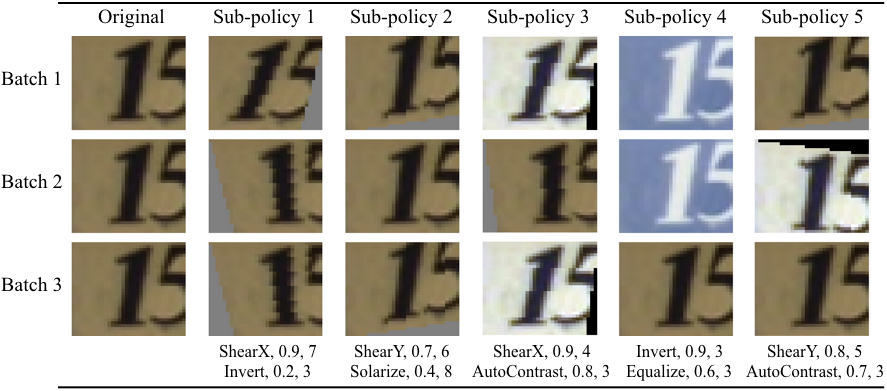
\includegraphics[width=\textwidth]{images/svhn_viz_policy2.png}
    \caption{Esempio di policy con 5 sub-policy, immagine tratta da \cite{DBLP:journals/corr/abs-1805-09501}}
    \label{fig:policy}
\end{figure} 
In totale le operazioni nello spazio di ricerca sono 16, ed ognuna di esse ha un intervallo di potenza discretizzato con cui può essere applicata che varia da $1$ a $10$. In maniera del tutto similare vengono discretizzati anche i valori di probabilità in un intervallo di $11$. Trovare quindi una subpolicy è un problema di ricerca in uno spazio di dimensione $(16 \times 10 \times 11)^2$. Considerando che una policy contiene $5$ subpolicy lo spazio di ricerca arriva a $(16 \times 10 \times 11)^{10}$, che è nell'ordine di grandezza di $10^{32}$.

L'algoritmo di ricerca prende spunto dalle tecniche di apprendimento per rinforzo. Le sue componenti sono due, il controller \ac{RNN} e l'algoritmo di addestramento, che in questo caso è il \textit{Proximal Policy Optimization} \cite{DBLP:journals/corr/SchulmanWDRK17}. L'addestramento del controller \ac{RNN} è realizzato con un segnale di ricompensa che rappresenta il miglioramento in termini di generalizzazione della rete child addestrata con la policy $S$. Nel caso di Figura \ref{fig:AutoAugment} la ricompensa è $R$, ovvero il risultato della valutaizone sul validation set. Alla fine di questa fase di ricerca vengono trovate le migliori $5$ policy, che vengono concatenate in un'unica grande policy contentente $25$ subpolicy.
\paragraph{AutoAugment per Object Detection}
Fino ad ora abbiamo parlato di \textit{AutoAugment} in termini di classificazione di una immagini, lo scopo della tesi è però realizzare \textit{Object Detection}. Gli stessi autori di \cite{DBLP:journals/corr/abs-1805-09501} in \cite{DBLP:journals/corr/abs-1906-11172} hanno evoluto questa tecnica per far si che operi anche su questo tipo di compiti.

Come in precedenza il problema viene trattato come una ricerca in uno spazio discreto. Sempre come prima vengono definite policy come insiemi di $K$ subpolicy, con queste ultime composte da $N$ operazioni da applicare all'immagine in maniera sequenziale. In maniera del tutto analoga ogni operazione ha una probabilità con cui sarà applicata, a differenza della classificazione è stata resa più granulare la scelta dei possibili valori discretizati, chiamandoli $M$ per la potenza e $L$ per la probabilità. 
Una importante differenza invece riguarda le operazioni che è possibile applicare all'immagine, in quanto in aggiunta alle classiche operazioni di trasformazione dell'intero frame si aggiungono ulteriori $6$ operazioni applicabili solamente a livello di \ac{BB}, raggiungendo così un totale di $22$ operazioni. La dimensione dello spazio di ricerca di una subpolicy raggiunge quindi le dimensioni di $(22 \times L \times M)^2$, e più in particolare lo spazio di ricerca di una policy arriva a $(22 \times L \times M)^{10}$.

Gli autori in esperimenti preliminari hanno trovato che porre $L = M = 6$ è un buon \textit{trade-off} tra performance e costi computazionali, in quanto si arriva ad uno spazio di ricerca nell'ordine di $10^{28}$. Purtroppo però rimane comunque computazionalmente molto oneroso in quanto con $400$ \ac{TPU} sono state impiegate circa $48$ ore. 

Tuttavia sono state rilasciate delle policy apprese da dataset differenti con cui sono stati eseguiti esperimenti che verranno successsivamente descritti. 
\subsection{Rand Augment}
\label{subsec:rand_augment}